\documentclass[10pt]{nsfcnsproposal}
\usepackage{url,graphicx,multirow,hyperref,wrapfig,subcaption,amsfonts,amsmath}
\usepackage[group-separator={,}]{siunitx}
\hypersetup{
  bookmarks=true,
  unicode=true,
  pdftoolbar=true,
  pdfmenubar=true,
  pdffitwindow=true,
  pdfstartview={FitV},
  pdftitle={},
  pdfauthor={},
  pdfnewwindow=true,
  colorlinks=false,
  pdfdisplaydoctitle=true,
  pdfborder={0 0 0},
  pdfinfo={
    Title={Another Great Proposal},
    Author={Geoffrey Challen},
  },
}
\usepackage[all]{hypcap}

\input{.xxxnote}
../common.tex
\pagestyle{plain}
\tightlists
\firmlists

\begin{document}

% 16 Nov 2010 : GWA : Summary is one page, no page number.

\chapterstyle{summary}
\pagenumbering{gobble}
% 16 Nov 2010 : GWA : One page. You know what to do.

\def\thetitle{Long Title}
\def\shorttitle{Title}
\def\theauthors{PI: \uline{Geoffrey Challen}\\\textit{SUNY Buffalo}}
\def\shortauthors{Challen}
\def\submissiondate{\today}

\chapter{\thetitle}

% <clean:start>
% <cc:start description="Summary" max=4400>

\textbf{\textsc{Keywords:}} (1) \textbf{keyword}; (2) \textbf{keyword}; (3)
\textbf{keyword}.

\textbf{\textsc{Intellectual Merit:}}

\textbf{\textsc{Broader Impacts:}}

% <cc:end>
% <clean:end>

\clearpage

% 16 Nov 2010 : GWA : Description is (usually) 15 pages, paginated.

\chapterstyle{proposal}
\pagenumbering{gobble}
\pagenumbering{arabic}

% 07 Oct 2011 : GWA : Insert sections here.

\chapter{Intellectual Merit}
\thispagestyle{empty}

% 16 Nov 2010 : GWA : Start with another punchy statement of the overall
%               goal.


% 16 Nov 2010 : GWA : What are the core research objectives of the project?
%               Break down into list or bullet format.

\section{Research Questions}
\label{section-researchquestions}

\begin{researchquestions}

\item Question one.

\label{Q1}

\item Question two.

\label{Q2}

\end{researchquestions}

\clearpage

\clearpage

% 06 Dec 2010 : GWA : Budget justification. Separate pagination.

\pagenumbering{gobble}
\pagenumbering{arabic}
\thispagestyle{empty}

% 14 Dec 2010 : GWA : Instructions: Budget Justification (Field K on the form)
%               Provide the required supporting information for the following
%               costs (See R&R Budget instructions): equipment; domestic and
%               foreign travel; participant/trainees; material and supplies;
%               publication; consultant services; ADP/computer services;
%               subaward/consortium/contractual; equipment or facility
%               rental/user fees; alterations and renovations; and indirect
%               cost type. Provide any other information you wish to submit
%               to justify your budget request. Attach a single budget
%               justification file for the entire project period in Field K.
%               The file automatically carries over to each budget year.

\section{Personnel}

\textbf{\textsc{Faculty Investigator:}}

\textbf{\textsc{Graduate Student Support:}} 
  
\textbf{\textsc{Undergraduate Research Assistants:}} 

\section{Travel}

\section{Material and Supplies}

\section{Computer Services}

\section{Tuition}

\section{Indirect Costs}

\clearpage

% 06 Dec 2010 : GWA : Facilities and equipment statement, separate
%               pagination.

\pagenumbering{gobble}
\pagenumbering{arabic}
\chapter{Facilities, Equipment, and Other Resources}
\chapter{Facilities, Equipment, and Other Resources}
\thispagestyle{empty}

% 03 Feb 2011 : GWA : Can be nice to have the new building here.

\begin{figure}[h!]
\centering
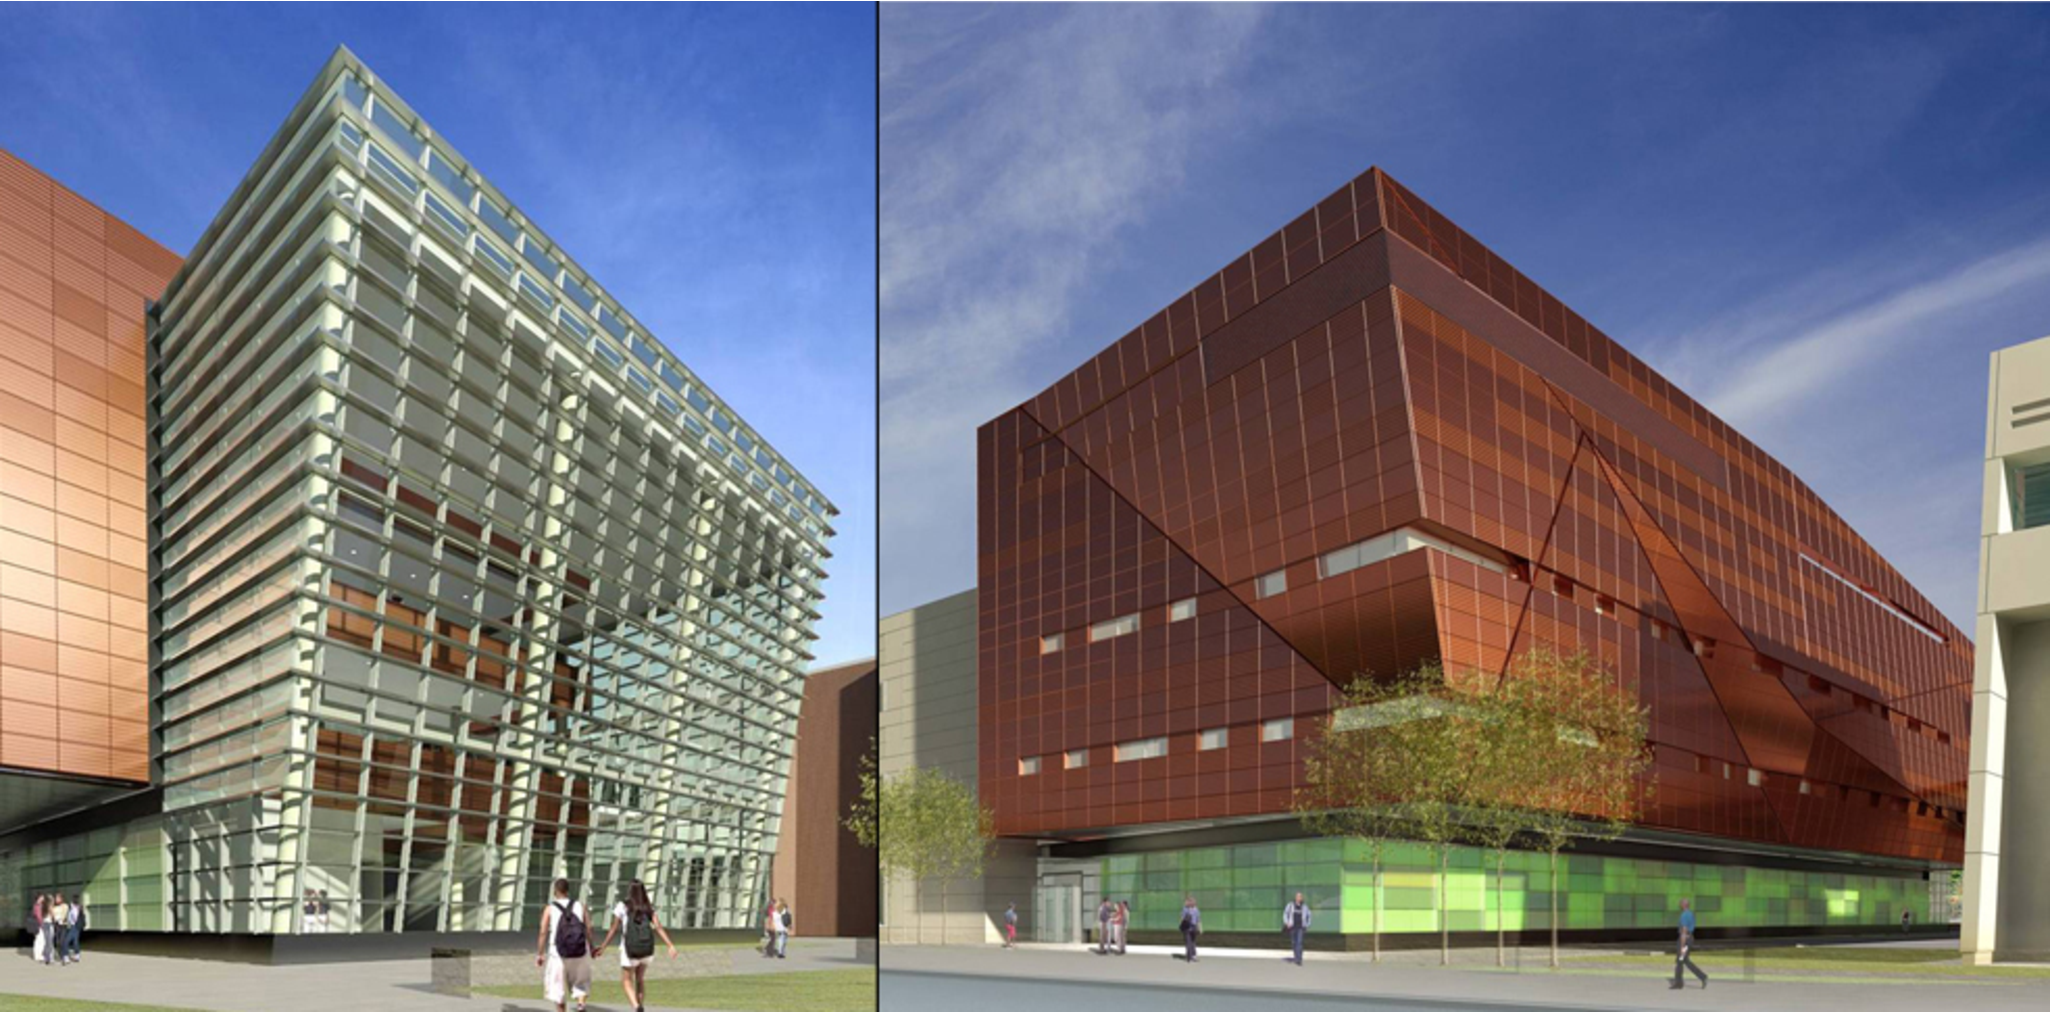
\includegraphics[width=\textwidth]{./figures/UBNewBuilding}
\caption{\textbf{New Davis UB Engineering Building}. The concept scheme shows the
SW elevation of the new \$75M Davis engineering building, scheduled to open in
summer 2011. (Image \copyright~Perkins Will.)}
\label{figure-newbuilding}
\end{figure}

\section{Facilities}

% 03 Feb 2011 : GWA : Standard departmental boilerplate.
%
% General research facilities include more than 200 i386 servers, x86\_64
% servers, SPARC-servers, PCs, and thin-client workstations. Available systems
% include three Dell Dimensions, thirty-four Dell Optiplexes, eight Dell
% PowerEdges, one Dell Precision, one Sun 5220, one Sun Blade 100, one Sun
% Blade 1000, one Sun Fire 280R, two Sun Fire V20Zs, more than 100 Sun Ray thin
% client terminals, and two Sun Ultra-60s. These systems are attached to a
% NetApp FAS2050A installed with 13 TB of disk space. Nine Dell Optiplex
% systems are configured as Linux and Windows student workstations. Laser
% printing resources are readily available. 

% 06 Dec 2010 : GWA : Use relevant descriptors.
%
%\textbf{\textsc{Laboratory:}}
%\textbf{\textsc{Clinical:}}
%\textbf{\textsc{Animal:}}
%\textbf{\textsc{Computer:}}
%\textbf{\textsc{Office:}}
%\textbf{\textsc{Other:}}

\section{Major Equipment}

% 03 Feb 2011 : GWA : Standard departmental boilerplate.
%
% Program-specific research facilities include 59 dedicated research systems.
% The Computer-Assisted Diagnostics Interventions Lab includes 23 systems, of
% which 18 members comprise a compute cluster connected to a 10 TB (installed)
% data storage device. The CyberInfrastructure Lab includes a 14-node compute
% cluster connected to a 15 TB (installed) data storage device. The
% Bioinformatics, Database, Data Mining, and Multimedia Group includes Dell and
% HP Oracle, MySQL, and compute servers. The Vision and Perceptual Machines Lab
% include two Apple Xserves. The 13 TB (installed) departmental
% network-attached storage device provides disk space for general and specific
% research projects.

\clearpage

% 16 Nov 2010 : GWA : References have no page limit, separate pagination.

\pagenumbering{gobble}
\pagenumbering{arabic}
\bibliography{references,geoffreychallen}
\bibliographystyle{plain}

\clearpage

% 16 Nov 2010 : GWA : Bio-sketches are limited to two pages each. Here they
%               are built together. Building under ./biosketches/ will build
%               them separately. Pagination is reset in biosketches.tex.

% 16 Nov 2010 : GWA : Biosketches for internal collaborators. Add yours in
%               ./biosketches/ following the template and then include it
%               here. Eventually these need to be built and uploaded
%               separately.

\setsecnumformat{}
\pagenumbering{arabic}
\chapterstyle{biosketch}
\setsecnumformat{\csname the#1\endcsname.\space}
\renewcommand{\thesection}{\Alph{section}}
\renewcommand{\thesubsection}{\roman{subsection}}

\chapter{Geoffrey Challen}

Geoffrey Challen (n\'{e} Werner-Allen)\\
Department of Computer Science and Engineering\\
University at Buffalo\\
338 Davis Hall\\
Buffalo, NY 14260-2500\\
\href{mailto:challen@buffalo.edu}{\texttt{challen@buffalo.edu}}\\
\url{http://www.cse.buffalo.edu/~challen/}

\section{Professional Preparation}

\begin{itemize}
\item Harvard University, Physics, A.B. 2003
\item Harvard University, Computer Science, Ph.D. 2010
\item Massachusetts Institute of Technology, Post-Doctoral Researcher, 2010-2011
\end{itemize}

\section{Appointments}

Assistant Professor, University at Buffalo, 07/15/2011--present.

\section{Products}

\subsection{Related Products}

\begin{enumerate}

\item \textbf{The Case for Power-Agile Computing}\\\uline{Geoffrey Challen}
and Mark Hempstead. In \emph{Proceedings of the 13th Workshop of Hot Topics
in Operating Systems (HotOS'11)}, May, 2011.
\nocite{poweragile-hotos11}

\item \textbf{IDEA: Integrated Distributed Energy Awareness for Wireless Sensor
Networks}\\ \uline{Geoffrey Werner Challen}, Jason Waterman and Matt Welsh. In
\emph{Proceedings of the 8th Annual International Conference on Mobile Systems,
Applications and Services (MobiSys'10)}, June, 2010.
\nocite{idea-mobisys10}

\item \textbf{Lance: Optimizing High-Resolution Data Collection in Wireless
Sensor Networks}\\ \uline{Geoffrey Werner-Allen}, Stephen Dawson-Haggerty and
Matt Welsh. In \emph{Proceedings of the Sixth ACM Conference on Embedded
Networked Sensor Systems (SenSys'08)}, November, 2008.
\nocite{lance-sensys08}

\item \textbf{PhoneLab: A Programmable Smartphone Testbed} (Invited Paper)\\
Anandatirtha Nandugudi, Anudipa Maiti, Taeyeon Ki, Fatih Bulut, Murat
Demirbas, Tevfik Kosar, Chunming Qiao, Steven Y. Ko and \uline{Geoffrey
Challen}. To appear in \emph{Proceedings of the First International Workshop
on Sensing and Big Data Mining (SenseMine'13)}, November, 2013.\\
\href{http://www.phone-lab.org}{\texttt{http://www.phone-lab.org}}. Online
public testbed. \nocite{phonelab-url,phonelab-sensemine13}

\item \textbf{\texttt{ops-class.org}: Operating Systems Education Online}\\
\href{http://www.ops-class.org}{\texttt{http://www.ops-class.org}}. Online
operating systems classroom supporting courses using the OS~161 educational
operating system.
\nocite{opsclass-url}

\end{enumerate}

\subsection{Significant Products}

\begin{enumerate}

\item \textbf{Mercury: A Wearable Sensor Network Platform for High-Fidelity
Motion Analysis}\\ Konrad Lorincz, Bor-rong Chen, \uline{Geoffrey Werner
Challen}, Atanu Roy Chowdhury, Shyamal Patel, Paolo Bonato and Matt Welsh. In
\emph{Proceedings of the Seventh ACM Conference on Embedded Networked Sensor
Systems (SenSys'09)}, November, 2009.
\nocite{mercury-sensys09}

\item \textbf{Peloton: Coordinated Resource Management for Sensor Networks}\\
Jason Waterman, \uline{Geoffrey Werner Challen}, and Matt Welsh. In
\emph{Proceedings of the 12th Workshop on Hot Topics in Operating Systems
(HotOS'09)}, May, 2009.
\nocite{peloton-hotos09}

\item \textbf{Resource Aware Programming in the Pixie OS}\\ Konrad Lorincz,
Bor-rong Chen, Jason Waterman, \uline{Geoff Werner-Allen} and Matt Welsh. In
\emph{Proceedings of the Sixth ACM Conference on Embedded Networked Sensor
Systems (SenSys'08)}, November, 2008.
\nocite{pixie-sensys08}

\item \textbf{Fidelity and Yield in a Volcano Monitoring Sensor Network}\\
\uline{Geoffrey Werner-Allen}, Konrad Lorincz, Jeff Johnson, Jonathan Lees and
Matt Welsh. In \emph{Proceedings of the Seventh USENIX Symposium on Operating
Systems Design and Implementation (OSDI'06)}, November, 2006.
\nocite{volcano-osdi06}

\item \textbf{Firefly-Inspired Sensor Network Synchronicity with Realistic
Radio Effects}\\ \uline{Geoffrey Werner-Allen}, Geetika Tewari, Ankit Patel,
Radhika Nagpal and Matt Welsh. In \emph{Proceedings of the Third ACM
Conference on Embedded Networked Sensor Systems (SenSys'05)}, November, 2005.
\nocite{firefly-sensys05}

\end{enumerate}

\section{Synergistic Activities}

\begin{itemize}

\item Program committee member: 11th ACM Conference on Embedded Networked
Sensor Systems (SenSys'13), Program committee member: 10th ACM Conference on
Embedded Networked Sensor Systems (SenSys'12), 9th ACM Conference on Embedded
Networked Sensor Systems (SenSys'11), 31st IEEE Real-Time Systems Symposium
(RTSS 2011) (Wireless Network Systems Track).

\item 2009-2010 Siebel Scholar.

\end{itemize}

\section{Collaborators \& Other Affiliations}

\subsection{Collaborators and Co-Editors}

Murat Demirbas (University at Buffalo), Mark Hempstead (Drexel University),
Branislav Kusy (CSIRO), Steven Y. Ko, Tevfik Kosar, Chunming Qiao (University
at Buffalo).

\subsection{Graduate Advisers and Postdoctoral Sponsors}

Matt Welsh (Google), Hari Balakrishnan (Massachusetts Institute of Technology).

\subsection{Thesis Adviser and Postgraduate-Scholar Sponsor}

Anand Nandugudi, Anudipa Maiti, Taeyeon Ki, Guru Prasad, Jinghao Shi
(University at Buffalo).

Total number of graduate students advised: 5; postgraduate-scholars
sponsored: 0.

% 16 Nov 2010 : GWA : All pubs follow.

%\item \textbf{Mercury: A Wearable Sensor Network Platform for High-Fidelity
%Motion Analysis}\\ Konrad Lorincz, Bor-rong Chen, \uline{Geoffrey Werner
%Challen}, Atanu Roy Chowdhury, Shyamal Patel, Paolo Bonato and Matt Welsh. In
%\emph{Proceedings of the Seventh ACM Conference on Embedded Networked Sensor
%Systems (SenSys’09)}, November, 2009.
%\nocite{mercury-sensys09}
%
%\item \textbf{Peloton: Coordinated Resource Management for Sensor Networks}\\
%Jason Waterman, \uline{Geoffrey Werner Challen}, and Matt Welsh. In
%\emph{Proceedings of the 12th Workshop on Hot Topics in Operating Systems
%(HotOS-XII)}, May, 2009.
%\nocite{peloton-hotos09}
%
%\item \textbf{Resource Aware Programming in the Pixie OS}\\ Konrad Lorincz,
%Bor-rong Chen, Jason Waterman, \uline{Geoff Werner-Allen} and Matt Welsh. In
%\emph{Proceedings of the Sixth ACM Conference on Embedded Networked Sensor
%Systems (SenSys’08)}, November, 2008.
%\nocite{pixie-sensys08}
%
%\item \textbf{Pixie: An Operating System for Resource-Aware Programming of
%Embedded Sensors}\\ Konrad Lorincz, Bor-rong Chen, Jason Waterman,
%\uline{Geoffrey Werner-Allen}, and Matt Welsh. In \emph{Proceedings of the
%Fifth Workshop on Embedded Networked Sensors (HotEmNets’08)}, June, 2008.
%\nocite{pixie-hotemnets08}
%
%\item \textbf{Fidelity and Yield in a Volcano Monitoring Sensor Network}\\
%\uline{Geoffrey Werner-Allen}, Konrad Lorincz, Jeff Johnson, Jonathan Lees and
%Matt Welsh. In \emph{Proceedings of the Seventh USENIX Symposium on Operating
%Systems Design and Implementation (OSDI’06)}, November, 2006.
%\nocite{volcano-osdi06}
%
%\item \textbf{Simulating the Power Consumption of Large-Scale Sensor Network
%Applications}\\ Victor Shnayder, Mark Hempstead, Bor-rong Chen, \uline{Geoff
%Werner-Allen} and Matt Welsh. In \emph{Proceedings of the Second ACM Conference
%on Embedded Networked Sensor Systems (SenSys’04)}, November, 2004.
%\nocite{powertossim-sensys04,

%\item \textbf{Firefly-Inspired Sensor Network Synchronicity with Realistic
%Radio Effects}\\ \uline{Geoffrey Werner-Allen}, Geetika Tewari, Ankit Patel,
%Radhika Nagpal and Matt Welsh. In \emph{Proceedings of the Third ACM Conference
%on Embedded Networked Sensor Systems (SenSys'05)}, November, 2005.
%\nocite{firefly-sensys05}
%
%\item \textbf{MoteLab: A Wireless Sensor Network Testbed}\\ \uline{Geoffrey
%Werner-Allen}, Pat Swieskowski, and Matt Welsh. In \emph{Proceedings of the
%Fourth International Conference on Information Processing in Sensor Networks
%(IPSN'05)}, April, 2005.
%\nocite{motelab-ipsn05}
%
%\item \textbf{Monitoring Volcanic Eruptions with a Wireless Sensor Network}\\
%\uline{Geoffrey Werner-Allen}, Jeff Johnson, Mario Ruiz, Jonathan Lees, and
%Matt Welsh. In \emph{Proceedings of the Second European Workshop on Wireless
%Sensor Networks (EWSN'05)}, January, 2005.
%\nocite{volcano-ewsn05}

\clearpage
\pagenumbering{arabic}
\chapter{My Collaborator}

My Collaborator\\
My Collaborator's University Address\\
Some University\\
Some City, Some State, Some Zip\\
\href{mailto:some@one.edu}{\texttt{some@one.edu}}\\
\url{http://www.some.edu/~one/}

\section{Professional Preparation}

\begin{itemize}
\item Awesome University, Awesome Degree, Awesome Time
\end{itemize}

\section{Appointments}

\section{Related Publications}

\begin{itemize}

\item \textbf{My Awesome Idea}\\ \uline{My Collaborator}, One of His Friends,
Another of His Friends. In \emph{Proceedings of the 8th Annual International
Conference on Awesomeness (AweTech’10)}, June, 2010.

\end{itemize}

\section{Other Significant Publications}

\begin{itemize}

\item \textbf{Another Awesome Idea}\\ \uline{My Collaborator}, One of His
Friends, Another of His Friends. In \emph{Proceedings of the 8th Annual
International Conference on Awesomeness (AweTech’10)}, June, 2010.

\end{itemize}

\section{Synergistic Activities}

\begin{itemize}

\item Program Committee Member, Best Conference Ever (BestSys'11).

\end{itemize}

\section{Ph.D. Thesis Adviser}

Some Guy (Affiliation).

\section{Post-Doctoral Supervisor}

Another Guy (Affiliation).

\section{Collaborators}

Cool Person One (Affiliation), Cool Person Two (Affilation).

\section{Former Ph.D. Students}

\clearpage


% 16 Dec 2010 : GWA : Project personnel statement.

\pagenumbering{gobble}
\pagenumbering{arabic}
\clearpage
% 17 Nov 2010 : List of personel, required by NSF.

\chapter{Project Personnel and Partner Institutions}
\thispagestyle{empty}

\begin{enumerate}

\item Geoffrey Challen; University at Buffalo; co-PI.

\end{enumerate}


% 24 Oct 2011 : GWA : Data management.

\pagenumbering{gobble}
\pagenumbering{arabic}
\clearpage
\chapter{Data Management Plan}
\thispagestyle{empty}


\end{document}
